\documentclass[11pt,a4paper]{article}
\usepackage[utf8]{inputenc}
\usepackage{amsmath, amssymb, amsthm}
\usepackage{geometry}
\usepackage{graphicx}
\usepackage{booktabs}
\usepackage{hyperref}
\usepackage{xcolor} % Required for defining custom colors
\usepackage{empheq} % Required for boxing numbered equations cleanly

\geometry{margin=1in}

\title{\textbf{Gaussian Distribution: Derivation, Mean, and Variance}}
\author{\textbf{Nishanka Das} \\ 
Department of Computer Science \\ 
Ramakrishna Mission Vivekananda Centenary College, Rahara
}

\date{\today}

% Define a command for the red box style
\newcommand{\redbox}[1]{\colorbox{red!10}{\setlength{\fboxrule}{1.2pt}\def\BorderColor{red}\fbox{#1}}}
% Alternative clean framework for empheq box
\newlength{\mytightbox}
\setlength{\mytightbox}{\fboxsep}

\begin{document}

\maketitle

\begin{center}
For any mistakes found please feel free to mail at: \\
\url{nishanka.das.rkmvcc@gmail.com}
\end{center}

\begin{abstract}
This document provides a rigorous and formal mathematical derivation of the Gaussian (Normal) probability density function following the historical framework proposed by Carl Friedrich Gauss in 1809. Furthermore, we explicitly evaluate the fundamental statistical properties of this distribution, demonstrating via improper calculus integration that its parameters $\mu$ and $\sigma^2$ correspond exactly to its mathematical mean and variance. An illustration of the Gaussian Distribution is mentioned in the figure. 
\begin{figure}[h]
\centering
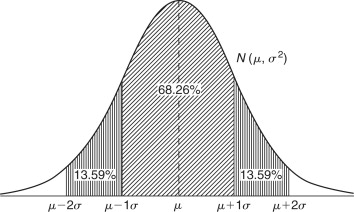
\includegraphics[scale=0.75]{abs}
\caption{Illustration of Gaussian Distribution}
\end{figure}
\end{abstract}

\section{Formal Derivation of the Gaussian Probability Density Function}
To derive the Gaussian distribution's mathematical form with rigorous formality, we follow the analytical framework established by Carl Friedrich Gauss, structured into five systematic stages.

\subsection{Formulating the Likelihood Function}
Let $X$ be a continuous random variable representing a true, unknown physical quantity. Let $\{x_1, x_2, \dots, x_n\}$ be a set of $n$ independent and identically distributed (i.i.d.) measurements of $X$. 

The true error $\varepsilon_i$ associated with each measurement $x_i$ is defined as:
\begin{equation}
\varepsilon_i = x_i - \theta
\end{equation}
where $\theta$ represents the true parameter value (the mean $\mu$).

Assuming there exists a continuous, differentiable probability density function (PDF), $f(\varepsilon)$, governing these errors, the joint probability density—known as the \textbf{Likelihood Function}, $L(\theta)$—is the product of their individual densities due to mutual independence:
\begin{equation}
L(\theta) = \prod_{i=1}^{n} f(x_i - \theta)
\end{equation}

\subsection{Applying the Principle of Maximum Likelihood}
The \textbf{Principle of Maximum Likelihood} asserts that the most mathematically sound estimate for the parameter $\theta$ is the one that maximizes the likelihood of observing the actual data sample obtained. To locate the critical point maximizing $L(\theta)$, we set its first derivative with respect to $\theta$ to zero. To simplify differentiation, we take the natural logarithm to obtain the \textbf{Log-Likelihood Function}, $\ln L(\theta)$:
\begin{equation}
\ln L(\theta) = \sum_{i=1}^{n} \ln f(x_i - \theta)
\end{equation}

Differentiating with respect to $\theta$ using the chain rule yields:
\begin{equation}
\frac{d}{d\theta}[\ln L(\theta)] = \sum_{i=1}^{n} \frac{f'(x_i - \theta)}{f(x_i - \theta)} \cdot (-1) = 0
\end{equation}

Multiplying by $-1$ and defining a kernel function $\phi(t) = \frac{f'(t)}{f(t)}$, our optimization condition reduces to:
\begin{equation}
\sum_{i=1}^{n} \phi(x_i - \theta) = 0
\end{equation}

\subsection{The Arithmetic Mean Constraint}
Gauss introduced the fundamental axiom that for any set of observations, the maximum likelihood estimator $\hat{\theta}$ must precisely equal the \textbf{arithmetic mean} ($\bar{x}$) of the sample:
\begin{equation}
\hat{\theta} = \bar{x} = \frac{1}{n}\sum_{i=1}^{n} x_i \implies \sum_{i=1}^{n} (x_i - \bar{x}) = 0
\end{equation}

For the conditions $\sum_{i=1}^{n} \phi(x_i - \bar{x}) = 0$ and $\sum_{i=1}^{n} (x_i - \bar{x}) = 0$ to hold simultaneously and universally for any arbitrary choice of sample size $n$ and measurements $x_i$, the function $\phi(t)$ must be directly proportional to its argument $t$:
\begin{equation}
\phi(t) = -k \cdot t
\end{equation}
where $k$ is a positive separation constant ($k > 0$) to satisfy the second-derivative test for a maximum, ensuring that probability decreases as the magnitude of the error increases.

\subsection{Solving the Functional Differential Equation}
Recalling the definition of $\phi(t)$, we establish a first-order separable ordinary differential equation:
\begin{equation}
\frac{f'(t)}{f(t)} = -kt
\end{equation}

Separating variables and integrating both sides:
\begin{equation}
\int \frac{1}{f(t)} \, df = \int -k t \, dt \implies \ln f(t) = -\frac{1}{2}kt^2 + C_0
\end{equation}

Exponentiating both sides yields:
\begin{equation}
f(t) = e^{C_0} \cdot e^{-\frac{1}{2}kt^2}
\end{equation}
Letting $A = e^{C_0}$ represent a positive constant of integration, and substituting back $t = x - \mu$ (where $\mu = \theta$), we find the structural form of the Gaussian function:
\begin{equation}
f(x) = A e^{-\frac{1}{2}k(x - \mu)^2}
\end{equation}

\subsection{Normalization and Determination of Constants}
To satisfy the axioms of probability, the total area under the curve over the entire real line domain must equal $1$:
\begin{equation}
\int_{-\infty}^{\infty} A e^{-\frac{1}{2}k(x - \mu)^2} \, dx = 1
\end{equation}

Letting $u = \sqrt{\frac{k}{2}}(x - \mu)$, it follows that $dx = \sqrt{\frac{2}{k}} \, du$. The integration becomes:
\begin{equation}
A \sqrt{\frac{2}{k}} \int_{-\infty}^{\infty} e^{-u^2} \, du = 1
\end{equation}
Knowing the standard Gaussian integral evaluates to $\int_{-\infty}^{\infty} e^{-u^2} \, du = \sqrt{\pi}$, we obtain:
\begin{equation}
A \sqrt{\frac{2\pi}{k}} = 1 \implies A = \sqrt{\frac{k}{2\pi}}
\end{equation}

By definition, the variance $\sigma^2$ of a continuous distribution is given by:
\begin{equation}
\sigma^2 = \int_{-\infty}^{\infty} (x - \mu)^2 f(x) \, dx = \sqrt{\frac{k}{2\pi}} \int_{-\infty}^{\infty} (x - \mu)^2 e^{-\frac{1}{2}k(x - \mu)^2} \, dx
\end{equation}
Evaluating this integral via integration by parts reveals the direct connection:
\begin{equation}
k = \frac{1}{\sigma^2}
\end{equation}
Substituting $k$ back into $A$ yields $A = \frac{1}{\sigma\sqrt{2\pi}}$, establishing the finalized Probability Density Function of the Normal Distribution. 

% Custom styled Red Box environment implementation around the final PDF equation:
\begin{empheq}[box={\fcolorbox{red}{white}}]{equation}
f(x) = \frac{1}{\sigma \sqrt{2\pi}} e^{-\frac{1}{2}\left(\frac{x-\mu}{\sigma}\right)^2}, \quad x \in (-\infty, \infty)
\end{empheq}

\section{Formal Derivation of the Mean}
The expected value, or mean, of a continuous random variable is defined as:
\begin{equation}
E[X] = \int_{-\infty}^{\infty} x \cdot f(x) \, dx = \int_{-\infty}^{\infty} x \cdot \frac{1}{\sigma \sqrt{2\pi}} e^{-\frac{1}{2}\left(\frac{x-\mu}{\sigma}\right)^2} \, dx
\end{equation}

We apply the linear substitution transformation:
\begin{equation}
u = \frac{x - \mu}{\sigma} \implies x = \sigma u + \mu \quad \text{and} \quad dx = \sigma \, du
\end{equation}
The integral becomes:
\begin{equation}
E[X] = \int_{-\infty}^{\infty} (\sigma u + \mu) \cdot \frac{1}{\sigma \sqrt{2\pi}} e^{-\frac{1}{2}u^2} (\sigma \, du) = \frac{1}{\sqrt{2\pi}} \int_{-\infty}^{\infty} (\sigma u + \mu) e^{-\frac{1}{2}u^2} \, du
\end{equation}

Expanding the linear terms via the linearity of integration:
\begin{equation}
E[X] = \frac{\sigma}{\sqrt{2\pi}} \int_{-\infty}^{\infty} u e^{-\frac{1}{2}u^2} \, du + \mu \cdot \frac{1}{\sqrt{2\pi}} \int_{-\infty}^{\infty} e^{-\frac{1}{2}u^2} \, du
\end{equation}

We evaluate the two integral terms independently:
\begin{enumerate}
    \item The integrand $g(u) = u e^{-\frac{1}{2}u^2}$ is a strict \textbf{odd function} ($g(-u) = -g(u)$). Over the symmetric domain $(-\infty, \infty)$, its integral evaluates to zero:
    \begin{equation}
    \int_{-\infty}^{\infty} u e^{-\frac{1}{2}u^2} \, du = 0
    \end{equation}
    \item The second integral represents the total area of the standard normal distribution, which equals $1$:
    \begin{equation}
    \frac{1}{\sqrt{2\pi}} \int_{-\infty}^{\infty} e^{-\frac{1}{2}u^2} \, du = 1
    \end{equation}
\end{enumerate}

Substituting these back into our expression:
\begin{empheq}[box={\fcolorbox{red}{white}}]{equation}
E[X] = \frac{\sigma}{\sqrt{2\pi}} \cdot (0) + \mu \cdot (1) = \mu
\end{empheq}
Thus, the parameter $\mu$ is formally proven to be the expected mathematical mean of the distribution.
\section{Formal Derivation of the Variance}
Alternatively, the variance can be computed more elegantly using the algebraic identity:
\begin{equation}
\text{Var}(X) = E[X^2] - (E[X])^2
\end{equation}

Since we have formally established that $E[X] = \mu$, we must evaluate the second raw moment, $E[X^2]$, defined as:
\begin{equation}
E[X^2] = \int_{-\infty}^{\infty} x^2 \cdot \frac{1}{\sigma \sqrt{2\pi}} e^{-\frac{1}{2}\left(\frac{x-\mu}{\sigma}\right)^2} \, dx
\end{equation}

Applying the linear substitution transformation $u = \frac{x - \mu}{\sigma} \implies x = \sigma u + \mu$ and $dx = \sigma \, du$, the integral becomes:
\begin{equation}
E[X^2] = \frac{1}{\sqrt{2\pi}} \int_{-\infty}^{\infty} (\sigma u + \mu)^2 e^{-\frac{1}{2}u^2} \, du
\end{equation}

Expanding the binomial term $(\sigma u + \mu)^2 = \sigma^2 u^2 + 2\mu\sigma u + \mu^2$ and applying the linearity of integration yields:
\begin{equation}
E[X^2] = \frac{\sigma^2}{\sqrt{2\pi}} \int_{-\infty}^{\infty} u^2 e^{-\frac{1}{2}u^2} \, du + \frac{2\mu\sigma}{\sqrt{2\pi}} \int_{-\infty}^{\infty} u e^{-\frac{1}{2}u^2} \, du + \frac{\mu^2}{\sqrt{2\pi}} \int_{-\infty}^{\infty} e^{-\frac{1}{2}u^2} \, du
\end{equation}

We evaluate each term independently:
\begin{enumerate}
    \item Utilizing integration by parts, the first integral evaluates to:
    \begin{equation}
    \frac{\sigma^2}{\sqrt{2\pi}} \int_{-\infty}^{\infty} u^2 e^{-\frac{1}{2}u^2} \, du = \frac{\sigma^2}{\sqrt{2\pi}} \cdot \sqrt{2\pi} = \sigma^2
    \end{equation}
    \item Because $g(u) = u e^{-\frac{1}{2}u^2}$ is an odd function, its integral over the symmetric domain vanishes:
    \begin{equation}
    \frac{2\mu\sigma}{\sqrt{2\pi}} \int_{-\infty}^{\infty} u e^{-\frac{1}{2}u^2} \, du = 0
    \end{equation}
    \item The total area of the standard normal kernel evaluates to unity:
    \begin{equation}
    \frac{\mu^2}{\sqrt{2\pi}} \int_{-\infty}^{\infty} e^{-\frac{1}{2}u^2} \, du = \mu^2 \cdot (1) = \mu^2
    \end{equation}
\end{enumerate}

Combining these individual components, we find the second raw moment to be:
\begin{equation}
E[X^2] = \sigma^2 + \mu^2
\end{equation}

Substituting $E[X^2]$ and $(E[X])^2 = \mu^2$ back into the foundational variance identity yields:
\begin{empheq}[box={\fcolorbox{red}{white}}]{equation}
\text{Var}(X) = (\sigma^2 + \mu^2) - \mu^2 = \sigma^2
\end{empheq}
Thus, the parameter $\sigma^2$ is verified as the true mathematical variance of the Gaussian distribution.
\end{document}